\section{紧致、可数紧致、列紧、序列紧致}\label{sec:7.3}

上两节介绍的 $A_{1}$, $A_{2}$, $T_{2}$, 连通性及道路连通性都是拓扑不变性, 即拓扑映射 (同胚) 下不变的性质. \cref{thm:7.2.7} 表明, 连通与道路连通还是连续不变性.

\begin{theorem}\label{thm:7.3.1}
设 $(X, \mathcal{T})$ 为拓扑空间.
\begin{enumerate}
  \item \textbf{紧致空间}: $X$ 的任何开覆盖必有有限子覆盖;

  \item \textbf{可数紧致空间}: $X$ 的任何可数开覆盖必有有限子覆盖;

  \item \textbf{列紧空间}: $X$ 的任何无限子集 $A$ 必有聚点 $a \in X$;

  \item \textbf{序列紧致空间}: $X$ 中每个点列 $\{x_{n}\}$ 必有收敛于 $x \in X$ 的子点列 $\{x_{n_{k}}\}$;

  \item 任何递降非空闭集序列 $\{F_{i}\}$ 必有交, 即 $\exists x \in \bigcap\limits_{n=1}^{\infty} F_{n}$ (或 $\bigcap\limits_{n=1}^{\infty} F_{n} \neq \varnothing$).
\end{enumerate}
它们具有如下关系:
\begin{center}
\begin{tikzpicture}[>=latex, x=1.5cm, y=1.5cm]
  \tikzset{
    node distance=0pt,
    nd/.style={inner sep=0pt, font=\normalsize},
    a/.style={line width=0.7pt, double, double distance=1.6pt, shorten <=3.5pt, shorten >=3.5pt,
              {Triangle[open, width=5pt, length=4pt]}-{Triangle[open, width=5pt, length=4pt]}},
    as/.style={line width=0.7pt, double, double distance=1.6pt, shorten <=3.5pt, shorten >=3.5pt,
               -{Triangle[open, width=5pt, length=4pt]}}
  }
  \node[nd] (n1) at (1.75, 1.75) {(1)};
  \node[nd] (n2) at (-0.25, 1.75) {(2)};
  \node[nd] (n3) at (-0.25, 0.05) {(3)};
  \node[nd] (n4) at (1.55, 0.05) {(4)};
  \node[nd] (n5) at (0.85, 0.85) {(5)};

  \draw[as] (n1) -- (n2);        % (1) => (2)
  \draw[as] (n2) -- (n3);        % (2) => (3)
  \draw[a]  (n2) -- (n5);        % (2) <=> (5)
  \draw[as] (n4) -- (n5);        % (4) => (5)
\end{tikzpicture}
\end{center}
\end{theorem}

\begin{proof}
(1) $\Rightarrow$ (2) 显然.

(2) $\Rightarrow$ (3) 设 $A$ 为 $X$ 的任一无限子集. 取 $A$ 的可数子集 $A_{1}$, 下证 $A_{1}$ 必有聚点 (属于 $X$), 当然它也是 $A$ 的聚点. (反证) 假设 $A_{1}$ 无聚点, 即 $A_{1}' = \varnothing \subset A_{1}$, 根据\cref{thm:7.1.5}(2), $A_{1}$ 为闭集. $\forall x \in A_{1}$, 由于 $x$ 不为 $A_{1}$ 的聚点, 故存在 $x$ 的开邻域 $U_{x}$, 使
\[
  U_{x} \cap (A_{1} \setminus \{x\}) = \varnothing,
\]
即
\[
  U_{x} \cap A_{1} = \{x\}.
\]
显然, $\{U_{x} \mid x \in A_{1}\} \cup \{A_{1}^{c}\}$ 为 $X$ 的可数开覆盖, 而 $(X, \mathcal{T})$ 为可数紧致空间, 故必存在有限子覆盖 $\{U_{x_{1}}, U_{x_{2}}, \cdots, U_{x_{n}}, A_{1}^{c}\}$. 因为 $A_{1}^{c}$ 中无 $A_{1}$ 的点, 所以 $\{U_{x_{1}}, U_{x_{2}}, \cdots, U_{x_{n}}\}$ 覆盖 $A_{1}$, 从而
\[
  A_{1} = \left(\bigcup_{i=1}^{n} U_{x_{i}}\right) \cap A_{1} = \bigcup_{i=1}^{n} \left(U_{x_{i}} \cap A_{1}\right) = \{x_{1}, x_{2}, \cdots, x_{n}\}
\]
为有限集, 这与 $A_{1}$ 为可数集相矛盾.

(2) $\Rightarrow$ (5) (反证) 假设 $\bigcap\limits_{n=1}^{\infty} F_{n} = \varnothing$, 则由 De Morgan 公式, 有
\[
  \bigcup_{n=1}^{\infty} F_{n}^{c} = \left(\bigcap_{n=1}^{\infty} F_{n}\right)^{c} = \varnothing^{c} = X.
\]
因此, $\{F_{n}^{c} \mid n \in \mathbb{Z}_{+}\}$ 为 $X$ 的可数开覆盖. 由 (2), 存在有限子覆盖 $\{F_{n_{1}}^{c}, F_{n_{2}}^{c}, \cdots, F_{n_{k}}^{c}\}$. 于是, 由
\[
  F_{n_{1}}^{c} \cup F_{n_{2}}^{c} \cup \cdots \cup F_{n_{k}}^{c} = X
\]
推出
\[
  \begin{aligned}
    \varnothing \neq F_{\max\{n_{1}, n_{2}, \cdots, n_{k}\}} &= F_{n_{1}} \cap F_{n_{2}} \cap \cdots \cap F_{n_{k}} \reason{De Morgan 公式} \left(F_{n_{1}}^{c} \cup F_{n_{2}}^{c} \cup \cdots \cup F_{n_{k}}^{c}\right)^{c} \\
    &= X^{c} = \varnothing.
  \end{aligned}
\]
矛盾. 所以, $\bigcap\limits_{n=1}^{\infty} F_{n} \neq \varnothing$.

(2) $\Leftrightarrow$ (5) 设 $\mathcal{I} = \{U_{n} \mid n \in \mathbb{Z}_{+}\}$ 为 $X$ 的任一可数开覆盖, 我们断定 $\mathcal{I}$ 必有有限子覆盖. (反证) 假设 $\mathcal{I}$ 无有限子覆盖. 令
\[
  F_{n} = \left(\bigcup_{i=1}^{n} U_{i}\right)^{c}, \quad n \in \mathbb{Z}_{+},
\]
则 $F_{n} \neq \varnothing$ (由 $\bigcup\limits_{i=1}^{n} U_{i} \neq X$), 且
\[
  F_{1} \supseteq F_{2} \supseteq \cdots \supseteq F_{n} \supseteq \cdots,
\]
由 (5) 得到
\[
  \varnothing \neq \bigcap_{n=1}^{\infty} F_{n} = \bigcap_{n=1}^{\infty} \left(\bigcup_{i=1}^{n} U_{i}\right)^{c} = \left(\bigcup_{n=1}^{\infty} \left(\bigcup_{i=1}^{n} U_{i}\right)\right)^{c} = \left(\bigcup_{n=1}^{\infty} U_{n}\right)^{c} = X^{c} = \varnothing,
\]
矛盾. 从而 $\mathcal{I}$ 有有限子覆盖, $(X, \mathcal{T})$ 是可数紧致的.

(4) $\Rightarrow$ (5) $\Leftrightarrow$ (2) 设 $\{F_{n}\}$ 为 $(X, \mathcal{T})$ 中任一递降非空闭集序列, 取 $x_{n} \in F_{n}$, $n \in \mathbb{Z}_{+}$, 因为 $X$ 是序列紧致的, 故存在 $\{x_{n}\}$ 的子点列 $\{x_{n_{i}}\}$ 收敛于 $x \in X$. 由于 $x_{n_{j}} \in F_{n_{i}}$ ($j = i, i+1, \cdots$), 以及 $F_{n_{i}}$ 为闭集, 所以, $x \in F_{n_{i}} \subset F_{i}$ ($i \in \mathbb{Z}_{+}$), 从而 $x \in \bigcap\limits_{n=1}^{\infty} F_{n}$. 这就证明了 $\bigcap\limits_{n=1}^{\infty} F_{n} \neq \varnothing$, (5) 成立.
\end{proof}

\begin{theorem}\label{thm:7.3.2}
对于度量空间 $(X, \rho)$ 诱导的拓扑空间 $(X, \mathcal{T}_{\rho})$, 关于\cref{thm:7.3.1}中的 (1)$\sim$(5), 有如下关系:
\begin{center}
\begin{tikzpicture}[>=latex, x=1.5cm, y=1.5cm]
  \tikzset{
    nd/.style={inner sep=0pt, font=\normalsize},
    a/.style={line width=0.7pt, double, double distance=1.6pt, shorten <=3.5pt, shorten >=3.5pt,
              {Triangle[open, width=5pt, length=4pt]}-{Triangle[open, width=5pt, length=4pt]}},
    as/.style={line width=0.7pt, double, double distance=1.6pt, shorten <=3.5pt, shorten >=3.5pt,
               -{Triangle[open, width=5pt, length=4pt]}}
  }
  \node[nd] (n1) at (1.75, 1.75) {(1)};
  \node[nd] (n2) at (-0.25, 1.75) {(2)};
  \node[nd] (n3) at (-0.25, 0.05) {(3)};
  \node[nd] (n4) at (1.75, 0.05) {(4)};
  \node[nd] (n5) at (0.75, 0.85) {(5)};

  \draw[a]  (n1) -- (n2);        % (1) <=> (2)
  \draw[as] (n2) -- (n3);        % (2) => (3)
  \draw[a]  (n2) -- (n5);        % (2) <=> (5)
  \draw[as] (n3) -- (n5);        % (3) => (5)
  \draw[as] (n3) -- (n4);        % (3) => (4)
  \draw[as] (n4) -- (n5);        % (4) => (5)
  \draw[as] (n4) -- (n1);        % (4) => (1)
\end{tikzpicture}
\end{center}
\end{theorem}

\begin{proof}
由\cref{thm:7.3.1}, 只需证明:

(3) $\Rightarrow$ (4) 设 $\{x_{n}\}$ 为 $(X, \mathcal{T}_{\rho})$ 中任一点列, 记 $A = \{x_{n} \mid n \in \mathbb{Z}_{+}\}$.

如果 $A$ 为有限集, 则 $\exists x \in A$, $n_{1} < n_{2} < \cdots < n_{k} < \cdots$, s. t. $x_{n_{k}} = x$. 于是
\[
  \lim_{k \to +\infty} x_{n_{k}} = x \in X.
\]
如果 $A$ 为无限集, 由于 $(X, \mathcal{T}_{\rho})$ 为列紧空间, $\exists x \in A'$. 令
\[
  A_{n} = \{x_{n}, x_{n+1}, \cdots\},
\]
\[
  n_{1} = \min\{j \mid x_{j} \in B(x; 1) \cap A_{1}\},
\]
\[
  n_{2} = \min\left\{j \;\middle|\; x_{j} \in B\left(x; \frac{1}{2}\right) \cap A_{n_{1}+1}\right\},
\]
\[
  \qquad \vdots
\]
\[
  n_{k} = \min\left\{j \;\middle|\; x_{j} \in B\left(x; \frac{1}{k}\right) \cap A_{n_{k-1}+1}\right\},
\]
\[
  \qquad \vdots
\]
显然, $x_{n_{k-1}} \notin A_{n_{k-1}+1}$, $n_{1} < n_{2} < \cdots < n_{k} < \cdots$, 从而 $\{x_{n_{k}}\}$ 为 $\{x_{n}\}$ 的一个子点列, 且 $x_{n_{k}} \in B\left(x; \frac{1}{k}\right)$, $0 \leqslant \rho\left(x_{n_{k}}, x\right) < \frac{1}{k} \to 0$ ($k \to +\infty$), 即 $\lim\limits_{k \to +\infty} x_{n_{k}} = x$. 这就证明了 $(X, \mathcal{T}_{\rho})$ 是序列紧致的.

(4) $\Rightarrow$ (1) 设 $(X, \rho)$ 为序列紧致的度量空间, $\mathcal{I}$ 为 $X$ 的一开覆盖, 根据\cref{thm:7.4.4} (Lebesgue 数定理), 有 Lebesgue 数 $\lambda = \lambda(\mathcal{I}) > 0$. 令
\[
  \widetilde{\mathcal{I}} = \left\{B\left(x; \frac{\lambda}{3}\right) \;\middle|\; x \in X\right\},
\]
则开覆盖 $\widetilde{\mathcal{I}}$ 有有限子覆盖. (反证) 假设 $\widetilde{\mathcal{I}}$ 无有限子覆盖, 则 $\widetilde{\mathcal{I}}$ 的任何有限子族都不覆盖 $X$. 任取 $x_{1} \in X$, 因为 $\left\{B\left(x_{1}; \frac{\lambda}{3}\right)\right\}$ 不是 $X$ 的覆盖, 取 $x_{2} \in X \setminus B\left(x_{1}; \frac{\lambda}{3}\right)$. 假定已定义了 $x_{1}, x_{2}, \cdots, x_{n} \in X$ 满足: 若 $j > i$, 则 $x_{j} \notin B\left(x_{i}; \frac{\lambda}{3}\right)$ (即 $\rho\left(x_{i}, x_{j}\right) > \frac{\lambda}{3}$)$^{(*)}$. 由于
\[
  \left\{B\left(x_{1}; \frac{\lambda}{3}\right), B\left(x_{2}; \frac{\lambda}{3}\right), \cdots, B\left(x_{n}; \frac{\lambda}{3}\right)\right\}
\]
不是 $X$ 的覆盖, 故可取
\[
  x_{n+1} \in X \setminus \bigcup_{i=1}^{n} B\left(x_{i}; \frac{\lambda}{3}\right).
\]
易见, $x_{1}, x_{2}, \cdots, x_{n+1}$ 也满足 $^{(*)}$. 因此, 我们归纳定义了 $X$ 中的一个序列 $\{x_{n}\}$ 满足 $^{(*)}$. 可以断定 $\{x_{n}\}$ 无收敛子序列 (否则, 若有子序列收敛于 $x$, 则 $B\left(x; \frac{\lambda}{6}\right)$ 中必含 $\{x_{n}\}$ 的无限多个点, 这是不可能的. 因为 $\{x_{n}\}$ 中不同点的距离大于 $\frac{\lambda}{3}$, 但 $B\left(x; \frac{\lambda}{6}\right)$ 中任意两点的距离都小于 $\frac{\lambda}{3}$), 这与 $(X, \mathcal{T}_{\rho})$ 为序列紧致空间相矛盾. 这证明了 $\widetilde{\mathcal{I}}$ 有有限子覆盖.

设 $\widetilde{\mathcal{I}}$ 的有限子覆盖为 $\left\{B\left(y_{1}; \frac{\lambda}{3}\right), B\left(y_{2}; \frac{\lambda}{3}\right), \cdots, B\left(y_{n}; \frac{\lambda}{3}\right)\right\}$, 由 $\forall i, \exists A_{i} \in \mathcal{I}$, s.t. $B\left(y_{i}; \frac{\lambda}{3}\right) \subset A_{i}$. 易见, $\{A_{1}, A_{2}, \cdots, A_{n}\}$ 为 $\mathcal{I}$ 的有限子覆盖. 于是证明了 $(X, \mathcal{T}_{\rho})$ 为紧致空间.
\end{proof}

\begin{theorem}\label{thm:7.3.3}
在 $(X, \mathcal{T}_{\rho})$ 中, 如果 $A \subset X$ (作为子拓扑空间) 序列紧致 (或可数紧致或列紧或紧致), 则 $A$ 为 $(X, \mathcal{T}_{\rho})$ 中的有界闭集. 但反之不真.
\end{theorem}

\begin{proof}[证法 1]
(反证) 假设 $A$ 无界, 则 $\exists x_{n}, x_{0} \in A$, s. t. $\rho(x_{n}, x_{0}) \geqslant n$. 显然, $\{x_{n}\}$ 无收敛子列. 这与 $A$ 序列紧致相矛盾. 因此, $A$ 有界.

(反证) 假设 $A$ 不为闭集, 则 $\exists x_{n} \in A$, 它收敛于 $x$, 但 $x \notin A$. 当然, $\{x_{n}\}$ 的一切子列也收敛于 $x \notin A$. 从而 $A$ 不是序列紧致的, 这与已知 $A$ 序列紧致相矛盾. 因此, $A$ 为闭集.

进而, 根据\cref{thm:7.3.2}, 可数紧致或列紧或紧致必为序列紧致, 因此, 也能推得 $A$ 为 $(X, \mathcal{T}_{\rho})$ 中的有界闭集.
\end{proof}

如果 $(X, \mathcal{T}_{\rho})$ 紧致, 我们还有下面两个证法.

\begin{proof}[证法 2]
取一定点 $x \in A$. 显然, $\mathcal{I} = \{B(x; n) \mid n \in \mathbb{Z}_{+}\}$ 为 $A$ 的一个开覆盖, 由于 $A$ 紧致, 故 $\exists N \in \mathbb{Z}_{+}$, s.t. $B(x; N) = \bigcup\limits_{n=1}^{N} B(x; n) \supseteq A$, 这就证明了 $A$ 是有界的.

再证 $A$ 为闭集, 只需证 $A^{c}$ 为开集. 设 $p \in A^{c}$, $\forall q \in A$, 取 $0 < \delta(q) \leqslant \frac{1}{2}\rho(p, q)$, 则
\[
  B(q; \delta(q)) \cap B(p; \delta(q)) = \varnothing.
\]
于是, $\mathcal{I} = \{B(q; \delta(q)) \mid q \in A\}$ 为紧致集 $A$ 的一个开覆盖, 故存在 $A$ 的有限子覆盖
\[
  \mathcal{I}_{1} = \{B(q_{i}; \delta(q_{i})) \mid i = 1, 2, \cdots, K\}.
\]
因为
\[
  B(q_{i}; \delta(q_{i})) \cap B(p; \delta(q_{i})) = \varnothing, \quad i = 1, 2, \cdots, K,
\]
所以
\[
  \bigcup_{i=1}^{K} B(q_{i}; \delta(q_{i})) \quad \text{与} \quad U = \bigcap_{i=1}^{K} B(p; \delta(q_{i}))
\]
不相交, 从而 $A \cap U = \varnothing$, $p \in U \subset A^{c}$, 其中 $U$ 为开集. 由此知 $A^{c}$ 为开集.
\end{proof}

\begin{proof}[证法 3]
(反证) 假设 $A$ 不为闭集, 则 $A' \not\subset A$, 即 $\exists x_{0} \in A'$, 但 $x_{0} \notin A$. 于是, 存在相异点组成的集合 $\{x_{n} \mid n \in \mathbb{Z}_{+}\} \subset A$, s.t. $\lim\limits_{n \to +\infty} x_{n} = x_{0}$.

显然,
\[
  \left\{B\left(x; \frac{1}{2}\rho(x, x_{0})\right) \;\middle|\; x \in A\right\}
\]
为 $A$ 的一个开覆盖, 而且它无有限子覆盖, 这与 $A$ 紧致相矛盾. 这就证明了 $A$ 为闭集.
\end{proof}

反之不真. 例如, $X = (0, 1)$ 作为通常的 Euclid 直线 $(\mathbb{R}^{1}, \mathcal{T}_{\rho_{0}}^{1})$ 的子拓扑空间为有界闭集, 但开区间族 $\left\{\left(\frac{1}{n}, 1\right) \;\middle|\; n \in \mathbb{Z}_{+}\right\}$ 为 $(0, 1)$ 的一个可数开覆盖, 但它无有限子覆盖. 因此, $A = (0, 1)$ 非紧致、非可数紧致. 因为 $A = (0, 1)$ 中的无限子集 $\left\{\frac{1}{n+1} \;\middle|\; n \in \mathbb{Z}_{+}\right\}$ 无聚点属于 $A$, 所以 $A = (0, 1)$ 非列紧. 由于 $A = (0, 1)$ 中的点列 $\left\{\frac{1}{n+1}\right\}$ 在 $A = (0, 1)$ 中无任何收敛子序列, 故 $A = (0, 1)$ 非序列紧致.

\begin{theorem}[闭集套原理]\label{thm:7.3.4}
序列紧致 (或可数紧致或列紧或紧致) 度量空间 $(X, \mathcal{T}_{\rho})$ 中的递降非空闭集序列 $\{F_{n}\}$, $F_{1} \supset F_{2} \supset \cdots \supset F_{n} \supset F_{n+1} \supset \cdots$, 且 $F_{n}$ 的直径
\[
  d(F_{n}) = \operatorname{diam} F_{n} = \sup\{\rho(x', x'') \mid x', x'' \in F_{n}\} \to 0 \quad (n \to +\infty),
\]
则 $\exists_{1} x \in \bigcap\limits_{n=1}^{\infty} F_{n}$.
\end{theorem}

\begin{proof}
由\cref{thm:7.3.2}(5) 知, $\exists x \in \bigcap\limits_{n=1}^{\infty} F_{n}$.

再证惟一性. (反证) 假设 $\exists x_{1}, x_{2} \in X$, s.t. $x_{1}, x_{2} \in \bigcap\limits_{n=1}^{\infty} F_{n}$, 则
\[
  0 \leqslant \rho(x_{1}, x_{2}) \leqslant \operatorname{diam} F_{n} \to 0 \quad (n \to +\infty),
\]
从而 $\rho(x_{1}, x_{2}) = 0$, $x_{1} = x_{2}$, 即 $\exists_{1} x \in \bigcap\limits_{n=1}^{\infty} F_{n}$.
\end{proof}

\begin{corollary}\label{cor:7.3.1}
$(\mathbb{R}^{n}, \mathcal{T}_{\rho_{0}}^{n})$ 中的递降非空 $n$ 维闭区间 (即 $n$ 维闭长方体) $\{I_{n}\}$, $I_{1} \supset I_{2} \supset \cdots \supset I_{n} \supset I_{n+1} \supset \cdots$, 且 $\operatorname{diam} I_{n} \to 0$ ($n \to +\infty$), 则 $\exists_{1} x \in \bigcap\limits_{n=1}^{\infty} I_{n}$.
\end{corollary}

\begin{proof}
在\cref{thm:7.3.4}中, 取 $(X, \mathcal{T}_{\rho}) = (I_{1}, \mathcal{T}_{\rho_{0}}^{n}|_{I_{1}})$ 即得本推论的结论.
\end{proof}

\begin{definition}\label{def:7.3.1}
设 $\{x_{n}\}$ 为度量空间 $(X, \rho)$ 中的一个点列, 如果 $\forall \varepsilon > 0$, $\exists N \in \mathbb{Z}_{+}$, 当 $n, m > N$ 时, 有 $\rho(x_{n}, x_{m}) < \varepsilon$, 则称 $\{x_{n}\}$ 为 $(X, \rho)$ 中的 \textbf{Cauchy 点列}或\textbf{基本点列}.

Cauchy 点列等价于: 如果 $\forall \varepsilon > 0$, $\exists N \in \mathbb{Z}_{+}$, 当 $n > N$ 时, $\forall p \in \mathbb{Z}_{+}$, 有 $\rho(x_{n}, x_{n+p}) < \varepsilon$.

如果 $(X, \rho)$ 中的任何 Cauchy (基本) 点列都收敛 (于 $X$ 中的点), 则称 $(X, \rho)$ 为\textbf{完备度量 (距离) 空间}.
\end{definition}

\begin{theorem}\label{thm:7.3.5}
(1) $(\mathbb{R}^{n}, \rho_{0}^{n})$ 为完备度量空间;

(2) 序列紧致 (或可数紧致, 或列紧, 或紧致) 度量空间 $(X, \mathcal{T}_{\rho})$ 是完备度量空间.
\end{theorem}

\begin{proof}
(1) 因为
\[
  |x_{i}^{m} - x_{i}^{m+p}| \leqslant \rho_{0}^{n}(x^{m}, x^{m+p}) \leqslant \sqrt{n} \max_{1 \leqslant i \leqslant n} |x_{i}^{m} - x_{i}^{m+p}|, \quad i = 1, 2, \cdots, n,
\]
所以 $\{x^{m}\}$ 为 $(\mathbb{R}^{n}, \rho_{0}^{n})$ 中的 Cauchy (基本) 点列 $\iff$ $\{x_{i}^{m}\}$ 为 $(\mathbb{R}^{1}, \rho_{0}^{1})$ 中的 Cauchy (基本) 数列 $\iff$ $\{x_{i}^{m}\}$ 在 $(\mathbb{R}^{1}, \rho_{0}^{1})$ ($i = 1, 2, \cdots, n$) 中均收敛 $\iff$ $\{x^{m}\}$ 在 $(\mathbb{R}^{n}, \rho_{0}^{n})$ 中收敛.

这就证明了 $(\mathbb{R}^{n}, \rho_{0}^{n})$ 为完备度量空间.

(2) 设 $\{x_{n}\}$ 为序列紧致度量空间 $(X, \mathcal{T}_{\rho})$ 的 Cauchy (基本) 点列, 则 $\{x_{n}\}$ 必有收敛子列 $\{x_{n_{k}}\}$, 记 $\lim\limits_{k \to +\infty} x_{n_{k}} = x_{0}$. $\forall \varepsilon > 0$, $\exists N \in \mathbb{Z}_{+}$, 当 $n, m > N$, $k > N$ 时,
\[
  \rho(x_{n}, x_{m}) < \frac{\varepsilon}{2}, \quad \rho(x_{n_{k}}, x_{0}) < \frac{\varepsilon}{2}.
\]
于是,
\[
  \rho(x_{n}, x_{0}) \leqslant \rho(x_{n}, x_{n_{k}}) + \rho(x_{n_{k}}, x_{0}) < \frac{\varepsilon}{2} + \frac{\varepsilon}{2} = \varepsilon.
\]
这就证明了 $\{x_{n}\}$ 收敛于 $x_{0} \in X$. 从而 $(X, \mathcal{T}_{\rho})$ 为完备度量空间.
\end{proof}

\begin{example}\label{ex:7.3.1}
对 $(\mathbb{R}^{n}, \rho_{0}^{n})$, \cref{thm:7.3.1}(5) 的结论并不成立. 只需取
\[
  F_{m} = [m, +\infty)^{n} = \underbrace{[m, +\infty) \times [m, +\infty) \times \cdots \times [m, +\infty)}_{n \text{ 个}},
\]
显然 $\{F_{m}\}$ 为递降非空闭集序列, 但 $\bigcap\limits_{m=1}^{\infty} F_{m} = \varnothing$.
\end{example}

\begin{theorem}\label{thm:7.3.6}
设 $A$ 为 $(\mathbb{R}^{n}, \mathcal{T}_{\rho_{0}}^{n})$ 的子拓扑空间, 则对于\cref{thm:7.3.1}中的 (1)$\sim$(5) 及下面的 (6) 满足以下关系:
\begin{center}
\begin{tikzpicture}[>=latex, x=1.5cm, y=1.5cm]
  \tikzset{
    nd/.style={inner sep=0pt, font=\normalsize},
    a/.style={line width=0.7pt, double, double distance=1.6pt, shorten <=3.5pt, shorten >=3.5pt,
              {Triangle[open, width=5pt, length=4pt]}-{Triangle[open, width=5pt, length=4pt]}},
    as/.style={line width=0.7pt, double, double distance=1.6pt, shorten <=3.5pt, shorten >=3.5pt,
               -{Triangle[open, width=5pt, length=4pt]}}
  }
  \node[nd] (n1) at (1.85, 1.75) {(1)};
  \node[nd] (n2) at (-0.25, 1.75) {(2)};
  \node[nd] (n3) at (-0.25, 0.05) {(3)};
  \node[nd] (n4) at (1.85, 0.05) {(4)};
  \node[nd] (n5) at (0.75, 0.85) {(5)};
  \node[nd] (n6) at (3.25, 0.9) {(6)};

  \draw[as] (n1) -- (n2);        % (1) => (2)
  \draw[a]  (n2) -- (n5);        % (2) <=> (5)
  \draw[as] (n2) -- (n3);        % (2) => (3)
  \draw[as] (n3) -- (n5);        % (3) => (5)
  \draw[as] (n3) -- (n4);        % (3) => (4)
  \draw[as] (n4) -- (n5);        % (4) => (5)
  \draw[a]  (n1) -- (n6);        % (1) <=> (6)
  \draw[a]  (n4) -- (n6);        % (4) <=> (6)
\end{tikzpicture}
\end{center}
其中: (6) $A$ 是有界闭集.
\end{theorem}

\begin{proof}
(4) $\Rightarrow$ (6) 由\cref{thm:7.3.3}证法 1 推得.

(1) $\Rightarrow$ (6) 由\cref{thm:7.3.3}证法 2, 3 推得.

(1) $\Leftrightarrow$ (6) (Heine-Borel). 设 $n$ 维闭区间 ($n$ 维闭长方体) $I_{1} \supseteq A$. (反证) 假设 $A$ 非紧致, 则存在 $A$ 的开覆盖 $\{U_{\alpha} \mid \alpha \in \Gamma\}$, 它无有限子覆盖. 将 $I_{1}$ $2^{n}$ 等分 (\cref{fig:7.3.1}), 必有一等分 $I_{2} \subset I_{1}$, 使 $I_{2} \cap A$ 无有限子覆盖. 再将 $I_{2}$ $2^{n}$ 等分, 必有一等分 $I_{3} \subset I_{2}$, 使 $I_{3} \cap A$ 无有限子覆盖. 于是, 得到一串 $n$ 维闭区间的递降序列
\[
  I_{1} \supseteq I_{2} \supseteq \cdots \supseteq I_{m} \supseteq \cdots,
\]
且 $I_{m}$ 的直径 $\operatorname{diam} I_{m} \to 0$ ($m \to +\infty$). 根据闭集套 (或闭区间套) 原理 (\cref{thm:7.3.4}, \cref{cor:7.3.1}), $\exists_{1} x^{0} \in I_{m}$, $\forall m \in \mathbb{Z}_{+}$. 取 $x^{m} \in I_{m} \cap A$, 显然, $\{x^{m}\}$ 收敛于 $x^{0}$. 又因 $A$ 为闭集, 故 $x^{0} \in A$. 因为 $\{U_{\alpha} \mid \alpha \in \Gamma\}$ 为 $A$ 的开覆盖, 所以, $\exists N \in \mathbb{Z}_{+}$, 当 $m > N$ 时, $I_{m} \subset U_{\alpha_{0}}$, 即 $\{U_{\alpha_{0}}\}$ 为 $I_{m} \cap A$ 的有限子覆盖, 这与 $I_{m} \cap A$ 无有限子覆盖相矛盾. 这就证明了 $A$ 是紧致的.
\end{proof}

\begin{figure}[htbp]
  \centering
  \begin{tikzpicture}[>=latex, scale=0.95]
    % I_1 : 整个正方形
    \draw[thick] (-3, -3) rectangle (3, 3);
    \node at (-2.55, 2.5) {$I_{1}$};

    % A : 粗闭曲线 (光滑卵形), 完全落在 I_1 内部
    \draw[very thick]
      (-2.35, 0.1) .. controls (-2.5, 1.7) and (-1.3, 2.6) .. (0.2, 2.6)
                   .. controls (1.8, 2.6) and (2.4, 1.5) .. (2.3, 0.1)
                   .. controls (2.2, -1.5) and (1.0, -2.5) .. (-0.5, -2.45)
                   .. controls (-1.9, -2.4) and (-2.2, -1.4) .. (-2.35, 0.1);
    \node at (-0.35, -2.0) {$A$};

    % 等分线 : I_1 四等分, I_2 四等分, I_3 四等分
    \draw[thick] (-3, 0.5) -- (3, 0.5);
    \draw[thick] (0.5, -3) -- (0.5, 3);
    \draw[thick] (1.75, 0.5) -- (1.75, 3);
    \draw[thick] (0.5, 1.75) -- (3, 1.75);
    \draw[thick] (1.125, 0.5) -- (1.125, 1.75);
    \draw[thick] (0.5, 1.125) -- (1.75, 1.125);

    % I_m : 阴影小方块
    \fill[pattern=north east lines, pattern color=black!70] (0.5, 0.5) rectangle (1.125, 1.125);
    \draw[thick] (0.5, 0.5) rectangle (1.125, 1.125);

    % x^0
    \fill (0.58, 0.62) circle (1.5pt);
    \node[below left=-1pt] at (0.58, 0.62) {$x^{0}$};

    % U_{alpha_0}
    \draw[thick] (0.58, 0.62) circle (0.85);
    \node[below=1pt] at (1.75, 0.05) {$U_{\alpha_{0}}$};

    % 标签 I_2, I_3
    \node at (1.15, 2.78) {$I_{2}$};
    \node at (0.85, 1.6) {$I_{3}$};

    % 指向 I_m 的箭头
    \draw[->, thick] (3.6, 0.85) -- (1.2, 0.8);
    \node[right=1pt] at (3.6, 0.85) {$I_{m}$};
  \end{tikzpicture}
  \caption{}\label{fig:7.3.1}
\end{figure}

\begin{example}\label{ex:7.3.2}
$\mathbb{R}^{n}$ 在 $(\mathbb{R}^{n}, \mathcal{T}_{\rho_{0}}^{n})$ 中非紧致.
\end{example}

\begin{proof}[证法 1]
显然, $\mathcal{I} = \{B(0; n) \mid n \in \mathbb{Z}_{+}\}$ 为 $\mathbb{R}^{n}$ 的一个开覆盖, 但它无有限子覆盖. 因此, $\mathbb{R}^{n}$ 在 $(\mathbb{R}^{n}, \mathcal{T}_{\rho_{0}}^{n})$ 中非紧致.
\end{proof}

\begin{proof}[证法 2]
因为无限子集 $A = \{(n, 0, 0, \cdots, 0) \mid n \in \mathbb{Z}_{+}\}$ 无聚点, 故 $\mathbb{R}^{n}$ 在 $(\mathbb{R}^{n}, \mathcal{T}_{\rho_{0}}^{n})$ 中非列紧. 根据\cref{thm:7.3.1}, $\mathbb{R}^{n}$ 在 $(\mathbb{R}^{n}, \mathcal{T}_{\rho_{0}}^{n})$ 中非紧致.
\end{proof}

\begin{proof}[证法 3]
因为点列 $\{(n, 0, 0, \cdots, 0)\}$ 无收敛子列, 故 $\mathbb{R}^{n}$ 在 $(\mathbb{R}^{n}, \mathcal{T}_{\rho_{0}}^{n})$ 中非序列紧致, 从而非紧致.
\end{proof}

\begin{proof}[证法 4]
因为 $\mathbb{R}^{n}$ 无界, 根据\cref{thm:7.3.3}知, $\mathbb{R}^{n}$ 在 $(\mathbb{R}^{n}, \mathcal{T}_{\rho_{0}}^{n})$ 中非紧致.
\end{proof}

读者仔细考虑一下, 你最欣赏的是哪一个证法? 应该是证法 1, 它只需用到紧致的定义, 不需用到其他定理.

\begin{theorem}\label{thm:7.3.7}
设 $(X, \mathcal{T}_{1})$ 与 $(Y, \mathcal{T}_{2})$ 都为拓扑空间, $f\colon X \to Y$ 为连续映射.
\begin{enumerate}
  \item 如果 $(X, \mathcal{T}_{1})$ 紧致, 则 $f(X)$ 也紧致;

  \item 如果 $(X, \mathcal{T}_{1})$ 可数紧致, 则 $f(X)$ 也可数紧致;

  \item 如果 $(X, \mathcal{T}_{1})$ 序列紧致, 则 $f(X)$ 也序列紧致.
\end{enumerate}
\end{theorem}

\begin{proof}
(1) $f(X)$ 视作 $(Y, \mathcal{T}_{2})$ 的子拓扑空间. 由定义知 $f\colon X \to f(X)$ 也为连续映射. 设 $\mathcal{I}$ 为 $f(X)$ 的任一开覆盖, 根据\cref{thm:7.2.2}(2), $\{f^{-1}(V) \mid V \in \mathcal{I}\}$ 为 $X$ 的一个开覆盖. 由 $X$ 紧致, $\{f^{-1}(V) \mid V \in \mathcal{I}\}$ 有一个有限子覆盖 $\{f^{-1}(V_{i}) \mid V_{i} \in \mathcal{I}, i = 1, 2, \cdots, n\}$. 因为 $f(f^{-1}(V_{i})) = V_{i}$, 所以 $\mathcal{I}_{1} = \{V_{i} \mid i = 1, 2, \cdots, n\}$ 为 $f(X)$ 关于 $\mathcal{I}$ 的一个有限子覆盖. 这就证明了 $f(X)$ 为 $(Y, \mathcal{T}_{2})$ 的紧致子集.

(2) 仿 (1) 证明.

(3) 在 $f(X)$ 中任取点列 $\{y_{n}\}$, 令 $x_{n} \in X$, s.t. $f(x_{n}) = y_{n}$. 因为 $(X, \mathcal{T}_{1})$ 序列紧致, 故 $\{x_{n}\}$ 有收敛子列 $\{x_{n_{k}}\}$ 收敛于 $x_{0} \in X$. 再由 $f$ 在 $x_{0}$ 连续及\cref{cor:7.2.1}知, $\{y_{n_{k}}\} = \{f(x_{n_{k}})\}$ 收敛于 $f(x_{0}) \in f(X)$, 即 $\{y_{n}\}$ 在 $f(X)$ 中有收敛的子点列 $\{y_{n_{k}}\}$. 这就证明了 $f(X)$ 是序列紧致的.
\end{proof}

\begin{corollary}\label{cor:7.3.2}
设 $(X, \rho_{1})$ 与 $(Y, \rho_{2})$ 都为度量空间, $f\colon X \to Y$ 为连续映射. 如果 $(X, \mathcal{T}_{\rho_{1}})$ 序列紧致 (或可数紧致或列紧或紧致), 则 $f(X)$ 也序列紧致 (或可数紧致或列紧或紧致).
\end{corollary}

\begin{proof}
由\cref{thm:7.3.7}, 只需证明: 如果 $(X, \mathcal{T}_{\rho_{1}})$ 列紧, 根据\cref{thm:7.3.2}, $(X, \mathcal{T}_{\rho_{1}})$ 序列紧致. 从\cref{thm:7.3.7}(3) 知, $f(X)$ 也序列紧致. 再根据\cref{thm:7.3.2}, $f(X)$ 为 $(Y, \mathcal{T}_{\rho_{2}})$ 的列紧子集.
\end{proof}

从\cref{thm:7.3.7}可知, 紧致、可数紧致与序列紧致都是连续不变性, 也是拓扑不变性. 此外, 列紧虽然不是连续不变性 (为什么?), 但根据列紧定义可推得, 它是拓扑不变性.

下面我们再来研究几个重要定理.

\begin{theorem}\label{thm:7.3.8}
紧致拓扑空间 $(X, \mathcal{T})$ 的闭子集 $A$ 为紧致子集.
\end{theorem}

\begin{proof}
设 $\{U \cap A \mid U \in \mathcal{T}_{0} \subset \mathcal{T}\}$ 为 $A$ 的任一开覆盖, 则 $\mathcal{T}_{0} \cup \{A^{c}\}$ 为紧致空间 $(X, \mathcal{T})$ 的一个开覆盖, 故必有有限子覆盖 $\{U_{1}, U_{2}, \cdots, U_{n}, A^{c}\}$. 由 $A \cap A^{c} = \varnothing$, 所以 $\{U_{1}, U_{2}, \cdots, U_{n}\}$ 覆盖 $A$, 即 $\{U_{1} \cap A, U_{2} \cap A, \cdots, U_{n} \cap A\}$ 覆盖 $A$, 它是 $\{U \cap A \mid U \in \mathcal{T}_{0} \subset \mathcal{T}\}$ 的有限子覆盖. 这就证明了 $A$ 为紧致子集.
\end{proof}

\begin{theorem}\label{thm:7.3.9}
$T_{2}$ 空间 $(X, \mathcal{T})$ 中的紧致子集 $A$ 为闭子集.
\end{theorem}

\begin{proof}
取 $p \in A^{c}$, $\forall q \in A$, 由于 $(X, \mathcal{T})$ 为 $T_{2}$ 空间, 故存在 $q$ 的开邻域 $U_{q}$ 与 $p$ 的开邻域 $V_{p}$, 使得 $U_{q} \cap V_{p} = \varnothing$. 易见, $\mathcal{I} = \{U_{q} \mid q \in A\}$ 为紧致子集 $A$ 的一个开覆盖, 它必有有限子覆盖 $\mathcal{I}_{1} = \{U_{q_{1}}, U_{q_{2}}, \cdots, U_{q_{n}}\}$. 令
\[
  U = \bigcup_{i=1}^{n} U_{q_{i}}, \quad V = \bigcap_{i=1}^{n} V_{p_{i}}.
\]
由于 $U_{q_{i}} \cap V \subset U_{q_{i}} \cap V_{p_{i}} = \varnothing$, 故 $U_{q_{i}} \cap V = \varnothing$,
\[
  U \cap V = \left(\bigcup_{i=1}^{n} U_{q_{i}}\right) \cap V = \bigcup_{i=1}^{n} \left(U_{q_{i}} \cap V\right) = \bigcup_{i=1}^{n} \varnothing = \varnothing,
\]
\[
  A \cap V = \varnothing, \quad p \in V \subset A^{c}.
\]
这就证明了 $A^{c}$ 为开集, 而 $A$ 为闭集.
\end{proof}

\begin{example}\label{ex:7.3.3}
设 $X = \{a, b\}$, $a \neq b$. $\mathcal{T}_{\text{平庸}} = \{\varnothing, X\}$. 由于 $\mathcal{T}_{\text{平庸}}$ 中只含两个元素, 故 $A = \{a\}$ 为紧致子集. 但它显然不为 $(X, \mathcal{T}_{\text{平庸}})$ 中的闭集.
\end{example}

\begin{theorem}\label{thm:7.3.10}
设 $(X, \mathcal{T}_{1})$ 为紧致空间, $(Y, \mathcal{T}_{2})$ 为 $T_{2}$ 空间, $f\colon X \to Y$ 为一一连续映射, 则 $f$ 为同胚.
\end{theorem}

\begin{proof}
设 $F$ 为 $(X, \mathcal{T}_{1})$ 中任一闭集, 因为 $(X, \mathcal{T}_{1})$ 为紧致空间, 根据\cref{thm:7.3.8}, 闭集 $F$ 也紧致. 由 $f$ 为连续映射及\cref{thm:7.3.7}(1) 知 $(f^{-1})^{-1}(F) = f(F)$ 也是紧致的. 从\cref{thm:7.3.9}可知, $T_{2}$ 空间 $(Y, \mathcal{T}_{2})$ 中的紧致子集 $f(F)$ 为闭子集. 由\cref{thm:7.2.2}(3) 立即推出 $f^{-1}$ 为连续映射, 而 $f$ 以及 $f^{-1}$ 都为同胚.
\end{proof}

\begin{example}\label{ex:7.3.4}
设 $X = [0, 2\pi)$ 为实直线 $(\mathbb{R}^{1}, \mathcal{T}_{\rho_{0}}^{1})$ 的子拓扑空间. 单位圆 $Y = S^{1}$ 为平面 $(\mathbb{R}^{2}, \mathcal{T}_{\rho_{0}}^{2})$ 的子拓扑空间. $f\colon X = [0, 2\pi) \to S^{1} = Y$, $\theta \mapsto f(\theta) = (\cos\theta, \sin\theta)$, 显然, $f$ 为一一连续映射. 但 $f^{-1}$ 在 $(\cos 0, \sin 0) = (1, 0)$ 处不连续, 从而 $f$ 不为同胚. 事实上, 对 $f^{-1}((1, 0)) = 0$ 的开邻域 $U_{0} = [0, \pi)$, 都不存在 $(1, 0)$ 的开邻域 $V$, 使得 $f^{-1}(V) \subset U_{0} = [0, \pi)$, 所以 $f^{-1}$ 在 $(1, 0)$ 不连续 (\cref{fig:7.3.2}).

\begin{figure}[htbp]
  \centering
  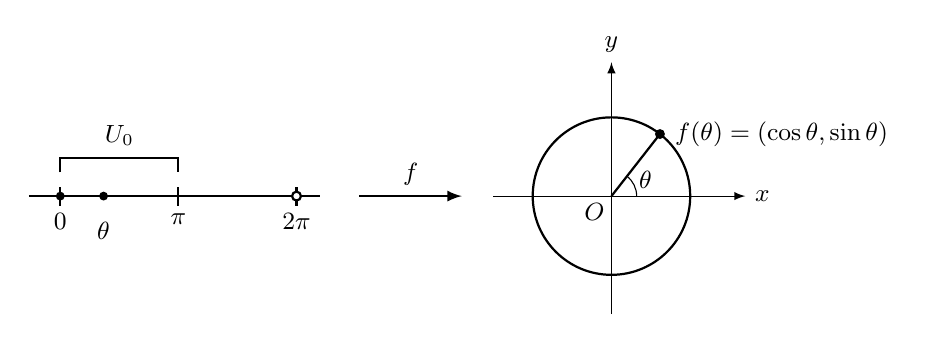
\begin{tikzpicture}[>=latex, scale=1.0]
    % 左: 实直线上的区间 [0, 2pi)
    \draw[thick] (-0.4, 0) -- (3.3, 0);
    \draw[thick] (0, -0.12) -- (0, 0.12) node[below=6pt] {\small $0$};
    \draw[thick] (1.5, -0.12) -- (1.5, 0.12) node[below=6pt] {\small $\pi$};
    \draw[thick] (3.0, -0.12) -- (3.0, 0.12) node[below=6pt] {\small $2\pi$};
    \fill (0, 0) circle (1.6pt);
    \draw[fill=white, thick] (3.0, 0) circle (1.6pt);
    \fill (0.55, 0) circle (1.6pt) node[below=6pt] {\small $\theta$};

    % U_0 的上方括号
    \draw[thick] (0, 0.3) -- (0, 0.48) -- (1.5, 0.48) -- (1.5, 0.3);
    \node[above=1pt] at (0.75, 0.48) {\small $U_{0}$};

    % 箭头 f
    \draw[->, thick] (3.8, 0) -- node[above] {\small $f$} (5.1, 0);

    % 右: 单位圆 S^1
    \begin{scope}[shift={(7.0, 0)}]
      \draw[->] (-1.5, 0) -- (1.7, 0) node[right] {\small $x$};
      \draw[->] (0, -1.5) -- (0, 1.7) node[above] {\small $y$};
      \node[below left=-1pt] at (0, 0) {\small $O$};

      \draw[thick] (0, 0) circle (1.0);

      \coordinate (P) at (52:1.0);
      \draw[thick] (0, 0) -- (P);
      \fill (P) circle (1.8pt);
      \node[right=2pt] at (P) {\small $f(\theta) = (\cos\theta, \sin\theta)$};
      \draw (0.32, 0) arc (0:52:0.32);
      \node at (26:0.48) {\small $\theta$};
    \end{scope}
  \end{tikzpicture}
  \caption{}\label{fig:7.3.2}
\end{figure}
\end{example}

\begin{example}\label{ex:7.3.5}
设 $X = Y = \{a, b\}$, $a \neq b$. 显然, 恒同映射
\[
  f = \operatorname{Id}_{X}\colon (X, \mathcal{T}_{\text{离散}}) \to (X, \mathcal{T}_{\text{平庸}})
\]
为一一连续映射, 但 $f^{-1}$ 不连续, 从而 $f$ 不为同胚. 事实上, 对 $f^{-1}(a) = a \in X$ 的开邻域 $\{a\}$, $a \in Y$ 的开邻域只有 $Y = \{a, b\}$, 显然 $f^{-1}(Y) = \{a, b\} \not\subset \{a\}$. 因此, $f^{-1}$ 在 $a$ 处不连续.
\end{example}

细心的读者会注意到\cref{ex:7.3.4}中 $X = [0, 2\pi)$ 非紧致, \cref{ex:7.3.5}中 $(Y, \mathcal{T}_{\text{平庸}})$ 不是 $T_{2}$ 空间, 它们都不符合\cref{thm:7.3.10}的条件.

我们知道, 连通、道路连通、紧致、可数紧致、序列紧致、列紧都为拓扑不变性, 作为它的应用, 我们往往可以判别两个拓扑空间不同胚.

\begin{example}\label{ex:7.3.6}
(1) $(\mathbb{Z}_{+}, \mathcal{T}_{1}) \not\cong (\mathbb{R}, \mathcal{T}_{2})$;

(2) $S^{n} \not\cong \mathbb{R}^{m}$, 其中 $S^{n}$ 为通常的 $n$ 维单位球面, $\mathbb{R}^{m}$ 为通常的 $m$ 维 Euclid 空间;

(3) $S^{1} \not\cong S^{2}$, 其中 $S^{1}$ 为通常的单位圆, $S^{2}$ 为通常的二维单位球面;

(4) $X \not\cong S^{1}$, 其中 $S^{1}$ 为通常的单位圆, $X = \{(x, y) \mid (x^{2} + y^{2})^{2} = a^{2}(x^{2} - y^{2})\} \subset \mathbb{R}^{2}$ ($a > 0$) 为平面上的双纽线.
\end{example}

\begin{proof}
(1) (反证) 假设 $(\mathbb{Z}_{+}, \mathcal{T}_{1}) \cong (\mathbb{R}, \mathcal{T}_{2})$, 则存在同胚 $f\colon \mathbb{Z}_{+} \to \mathbb{R}$. 因此, $\mathbb{Z}_{+}$ 与 $\mathbb{R}$ 在 $f$ 下一一对应, 但 $\mathbb{Z}_{+}$ 可数, $\mathbb{R}$ 不可数, 矛盾.

(2) (反证) 假设 $S^{n} \cong \mathbb{R}^{m}$, 则存在同胚 $f\colon S^{n} \to \mathbb{R}^{m}$. 由于 $S^{n}$ 紧致, 而 $\mathbb{R}^{m}$ 非紧致, 这与紧致为拓扑不变性相矛盾.

(3) (反证) 假设 $S^{1} \cong S^{2}$, 则存在同胚 $f\colon S^{1} \to S^{2}$. 于是, $f\colon S^{1} \setminus \{(1, 0), (-1, 0)\} \to S^{2} \setminus \{f(1, 0), f(-1, 0)\}$ 也为同胚. 由于 $S^{1} \setminus \{(1, 0), (-1, 0)\}$ 不连通, 而 $S^{2} \setminus \{f(1, 0), f(-1, 0)\}$ 连通 (\cref{ex:7.2.4}), 这与连通性为拓扑不变性相矛盾.

(4) (反证) 假设 $X \cong S^{1}$, 则存在同胚 $f\colon X \to S^{1}$. 于是, $f\colon X \setminus \{(0, 0)\} \to S^{1} \setminus \{f(0, 0)\}$ 也为同胚. 由于 $X \setminus \{(0, 0)\}$ 不连通, 而 $S^{1} \setminus \{f(0, 0)\}$ 连通, 这与连通为拓扑不变性相矛盾.
\end{proof}


\begin{exblock}{练习题 7.3}

  \item 证明: $A$ 为 $(X, \mathcal{T})$ 的紧致子集 $\iff (X, \mathcal{T})$ 的任一闭集类 $\mathcal{F}_{0} \subset \mathcal{F}$, 且 $A \cap \left(\bigcap\limits_{F \in \mathcal{F}_{0}} F\right) = \varnothing$, 则有 $A_{1}, A_{2}, \cdots, A_{k} \in \mathcal{F}_{0}$, 使得 $A \cap \left(\bigcap\limits_{i=1}^{k} A_{i}\right) = \varnothing$.

  \item 证明: $A$ 为 $(X, \mathcal{T})$ 的可数紧致子集 $\iff (X, \mathcal{F})$ 的任一可数闭集类 $\mathcal{F}_{0} \subset \mathcal{F}$, 且 $A \cap \left(\bigcap\limits_{F \in \mathcal{F}_{0}} F\right) = \varnothing$, 则有 $A_{1}, A_{2}, \cdots, A_{k} \in \mathcal{F}_{0}$, 使得 $A \cap \left(\bigcap\limits_{i=1}^{k} A_{i}\right) = \varnothing$.

  \item 设 $P_{i}\colon \mathbb{R}^{2} \to \mathbb{R}^{1}$, $P_{i}(x_{1}, x_{2}) = x_{i}$ 为投影算子, $A \subset \mathbb{R}^{2}$ 为 $(\mathbb{R}^{2}, \mathcal{T}_{\rho_{0}}^{2})$ 中的紧致集. 证明:
  \begin{enumerate}
    \item $P_{i}$ 为连续映射;
    \item $P_{i}(A)$ 也为 $(\mathbb{R}^{1}, \mathcal{T}_{\rho_{0}}^{1})$ 中的紧致集.
  \end{enumerate}

  \item 设 $A, B \subset \mathbb{R}^{1}$. 证明: $A \times B$ 为 $(\mathbb{R}^{2}, \mathcal{T}_{\rho_{0}}^{2})$ 中的紧致集 $\iff$ $A$ 与 $B$ 均为 $(\mathbb{R}^{1}, \mathcal{T}_{\rho_{0}}^{1})$ 中的紧致集.

  \item 证明: 拓扑空间 $(X, \mathcal{T})$ 的任何有限子集都为紧致子集.

  \item 设 $\mathcal{T}'$ 与 $\mathcal{T}$ 都为 $X$ 的拓扑, 且 $\mathcal{T}' \subset \mathcal{T}$. 证明: 当 $(X, \mathcal{T})$ 紧致时, $(X, \mathcal{T}')$ 也紧致.

  \item 证明: 拓扑空间 $(X, \mathcal{T})$ 中任何有限个紧致子集的并集仍是一个紧致子集.

  \item 证明: 拓扑空间 $(X, \mathcal{T})$ 中任何一族紧致闭子集的交仍是一个紧致闭集.
\end{exblock}

\begin{exblock}{思考题 7.3}

  \item 在\cref{thm:7.3.2}中, 证明: (3) $\Rightarrow$ (5), (5) $\Rightarrow$ (4).

  \item 设 $(X, \mathcal{T})$ 为 $T_{2}$ 空间, $A \subset X$ 为 $(X, \mathcal{T})$ 中的紧致子集, $x \in A^{c}$. 证明: $x$ 与 $A$ 分别存在开邻域 $U$ 与 $V$, 使得 $U \cap V = \varnothing$.

  \item 设 $(X, \mathcal{T})$ 为 $T_{2}$ 空间, 如果 $A$ 与 $B$ 为 $(X, \mathcal{T})$ 的不交紧致子集, 则 $A$ 与 $B$ 分别存在开邻域 $U$ 与 $V$, 使得 $U \cap V = \varnothing$.

  \item 证明: $T_{2}$ 空间 $(X, \mathcal{T})$ 中任意多个紧致子集的交仍为紧致子集.

  \item 设 $(X, \rho)$ 为度量空间, $A$ 为 $(X, \mathcal{T}_{\rho})$ 的列紧子集. 证明: $A$ 为有界闭集.

  \item (1) 设 $(X, \rho)$ 为度量空间. $X$ 中的两个非空子集 $A$ 与 $B$ 的距离 $\rho(A, B)$ 定义为
  \[
    \rho(A, B) = \inf\{\rho(x, y) \mid x \in A, y \in B\}.
  \]
  当 $A = \{a\}$ 时, $\rho(a, B) = \rho(\{a\}, B) = \inf\{\rho(a, y) \mid y \in B\}$ 称为 $a$ 与集合 $B$ 之间的距离.

  证明:
  \begin{enumerate}
    \item 如果 $A$ 与 $B$ 为 $(X, \rho)$ 中的两个非空紧致子集, 则 $\exists a \in A$ 与 $b \in B$, s.t. $\rho(a, b) = \rho(A, B)$;

    \item 设 $X = \{-1\} \cup (0, 1)$ 作为 $(\mathbb{R}^{1}, \mathcal{T}_{\rho_{0}}^{1})$ 的子度量空间, $A = \{-1\}$ 与 $B = (0, 1)$ 分别为 $X$ 的紧致子集与闭集, 易见, 它无 (1) 中的结论;

    \item 设 $A$ 与 $B$ 分别为 $(\mathbb{R}^{n}, \rho_{0}^{n})$ 中的非空紧致子集与非空闭集, 则 $\exists a \in A$ 与 $b \in B$, s.t. $\rho_{0}^{n}(a, b) = \rho_{0}^{n}(A, B)$;

    \item 在 $(\mathbb{R}^{2}, \rho_{0}^{2})$ 中给出两个不相交的非空闲集 $A$ 与 $B$, 使得 $\rho_{0}^{2}(A, B) = 0$, 但不存在 $a \in A$, 不存在 $b \in B$, s.t. $\rho_{0}^{2}(a, b) = \rho_{0}^{2}(A, B)$;

    \item 设 $A$ 与 $B$ 分别为度量空间 $(X, \rho)$ 的非空紧子集与非空闭集. 证明:
    \[
      \rho(A, B) = 0 \iff A \cap B \neq \varnothing.
    \]
  \end{enumerate}

  \item 证明: 不存在由 $[0, 1]$ 到圆周上的一一连续映射.

  \item 证明: 不存在由 $[0, 1]$ 到 $[0, 1] \times [0, 1]$ 上的一一连续映射.

  \item 设 $E \subset \mathbb{R}^{n}$, $f\colon E \to \mathbb{R}^{m}$.
  \begin{enumerate}
    \item 如果 $E$ 为闭集, $f$ 连续, 则 $f$ 的图像
    \[
      G(f) = \{(x, f(x)) \mid x \in E\}
    \]
    为 $\mathbb{R}^{n+m}$ 中的闭集;

    \item 如果 $E$ 为紧致集, $f$ 连续, 则 $G(f)$ 也为紧致集;

    \item 如果 $G(f)$ 为紧致集, 则 $f$ 连续;

    \item 如果 $G(f)$ 为闭集, $f$ 是否连续?
  \end{enumerate}
\end{exblock}